% ╔══════════════════════════════════════════════════════════════════════════════╗
% ║  Understanding the impact of emulators in our inference pipelines          ║
% ║  AI in Radio Astronomy, Royal Observatory Edinburgh, March 2026            ║
% ║  Harry T. J. Bevins                                                        ║
% ╚══════════════════════════════════════════════════════════════════════════════╝
%
% Compile with: pdflatex emulator_accuracy.tex  (twice for refs/page numbers)
% Output:       emulator_accuracy.pdf

\documentclass[aspectratio=169, 12pt]{beamer}

% ─── Fonts ────────────────────────────────────────────────────────────────────
\usepackage[T1]{fontenc}
\usepackage{helvet}
\renewcommand{\familydefault}{\sfdefault}
\usepackage{microtype}

% ─── Math ─────────────────────────────────────────────────────────────────────
\usepackage{amsmath, amssymb}

% ─── Graphics & Layout ────────────────────────────────────────────────────────
\usepackage{graphicx}

% ─── Hyperlinks ───────────────────────────────────────────────────────────────
\usepackage{hyperref}
\hypersetup{colorlinks=true, urlcolor=blue, linkcolor=black, citecolor=black}

% ─── Colors ───────────────────────────────────────────────────────────────────
\usepackage{xcolor}
\definecolor{footergray}{RGB}{130, 130, 130}
\definecolor{accentblue}{RGB}{20, 40, 100}

% ══════════════════════════════════════════════════════════════════════════════
%  TALK METADATA
% ══════════════════════════════════════════════════════════════════════════════
\newcommand{\talkconfooter}{AI in Radio Astronomy, ROE Edinburgh, Mar 2026}
\newcommand{\talkemail}{htjb2@cam.ac.uk}
\newcommand{\talkarxiv}{\href{https://arxiv.org/abs/2503.13263}{arXiv:2503.13263}}

% ══════════════════════════════════════════════════════════════════════════════
%  BEAMER APPEARANCE
% ══════════════════════════════════════════════════════════════════════════════
\setbeamertemplate{navigation symbols}{}
\setbeamercolor{background canvas}{bg=white}
\setbeamercolor{normal text}{fg=black, bg=white}
\setbeamercolor{frametitle}{fg=black, bg=white}
\setbeamerfont{frametitle}{size=\large, series=\bfseries}
\setbeamertemplate{frametitle}{%
    \vspace{0.45em}\insertframetitle%
}
\setbeamercolor{item}{fg=black}
\setbeamercolor{subitem}{fg=black}
\setbeamertemplate{itemize item}{\small$\bullet$}
\setbeamertemplate{itemize subitem}{--}
\setlength{\leftmargini}{1.2em}
\let\olditemize\itemize
\renewcommand{\itemize}{\olditemize\setlength{\itemsep}{12pt}}

% ─── Footer ───────────────────────────────────────────────────────────────────
\setbeamertemplate{footline}{%
    \begin{beamercolorbox}[wd=\paperwidth, ht=2.4ex, dp=1.4ex]{footline}
        \hspace*{0.025\paperwidth}%
        {\color{footergray}\scriptsize\textbf{\talkconfooter{} -- \talkemail}}%
        \hfill
        {\color{blue}\scriptsize\talkarxiv}%
        \hspace{0.8em}%
        {\color{footergray}\scriptsize\insertframenumber}%
        \hspace*{0.025\paperwidth}%
    \end{beamercolorbox}%
}

% ─── Title page ───────────────────────────────────────────────────────────────
\setbeamertemplate{title page}{%
    \vspace{0.10\paperheight}
    \begin{center}
        {\bfseries\LARGE Understanding the impact of emulators\\[0.2em]
        in inference \par}
        \vspace{0.9em}
        {\large Harry T.\ J.\ Bevins\par}
        \vspace{0.25em}
        {\normalsize Kavli Fellow\par}
        \vspace{0.3em}
        {\small with Thomas Gessey-Jones, Will Handley\par}
        \vspace{1.3em}
        
\includegraphics[height=1.0cm]{../../beamer-template/logos/cambridge.png}\hspace{0.5cm}%
        
\includegraphics[height=1.0cm]{../../beamer-template/logos/kicc.png}\hspace{0.5cm}%
        
\includegraphics[height=1.0cm]{../../beamer-template/logos/cavendish.png}%
    \end{center}
}

% ─── Section divider ──────────────────────────────────────────────────────────
\newcommand{\sectionframe}[1]{%
    \begin{frame}{}
        \vfill
        \begin{center}{\large #1}\end{center}
        \vfill
    \end{frame}%
}

% ══════════════════════════════════════════════════════════════════════════════
\begin{document}
% ══════════════════════════════════════════════════════════════════════════════

% ── 1. Title slide ────────────────────────────────────────────────────────────
\begin{frame}{}
    \titlepage
\end{frame}

% ── 2a. Why emulators? ─────────────────────────────────────────────────────────
\begin{frame}{Emulators in astrophysics and cosmology}
    \begin{columns}[T]
        \begin{column}{0.55\textwidth}
            \vspace{1em}
            \begin{itemize}
                \item Our goal is to infer the nature of the Universe from observations
                \item This requires comparison of our observations $D$ to models $M(\theta)$
                \item Simulations take \textbf{minutes, hours or even days evaluate} per parameter set
                \item Bayesian inference requires $10^4$--$10^6$ evaluations
            \end{itemize}
        \end{column}
        \hfill
        \begin{column}{0.48\textwidth}
            \vspace{1em}
            \centering
            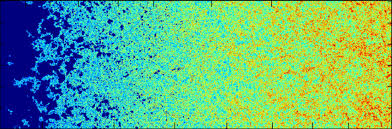
\includegraphics[width=\textwidth]{figs/21-cm-lightcone.jpeg}
            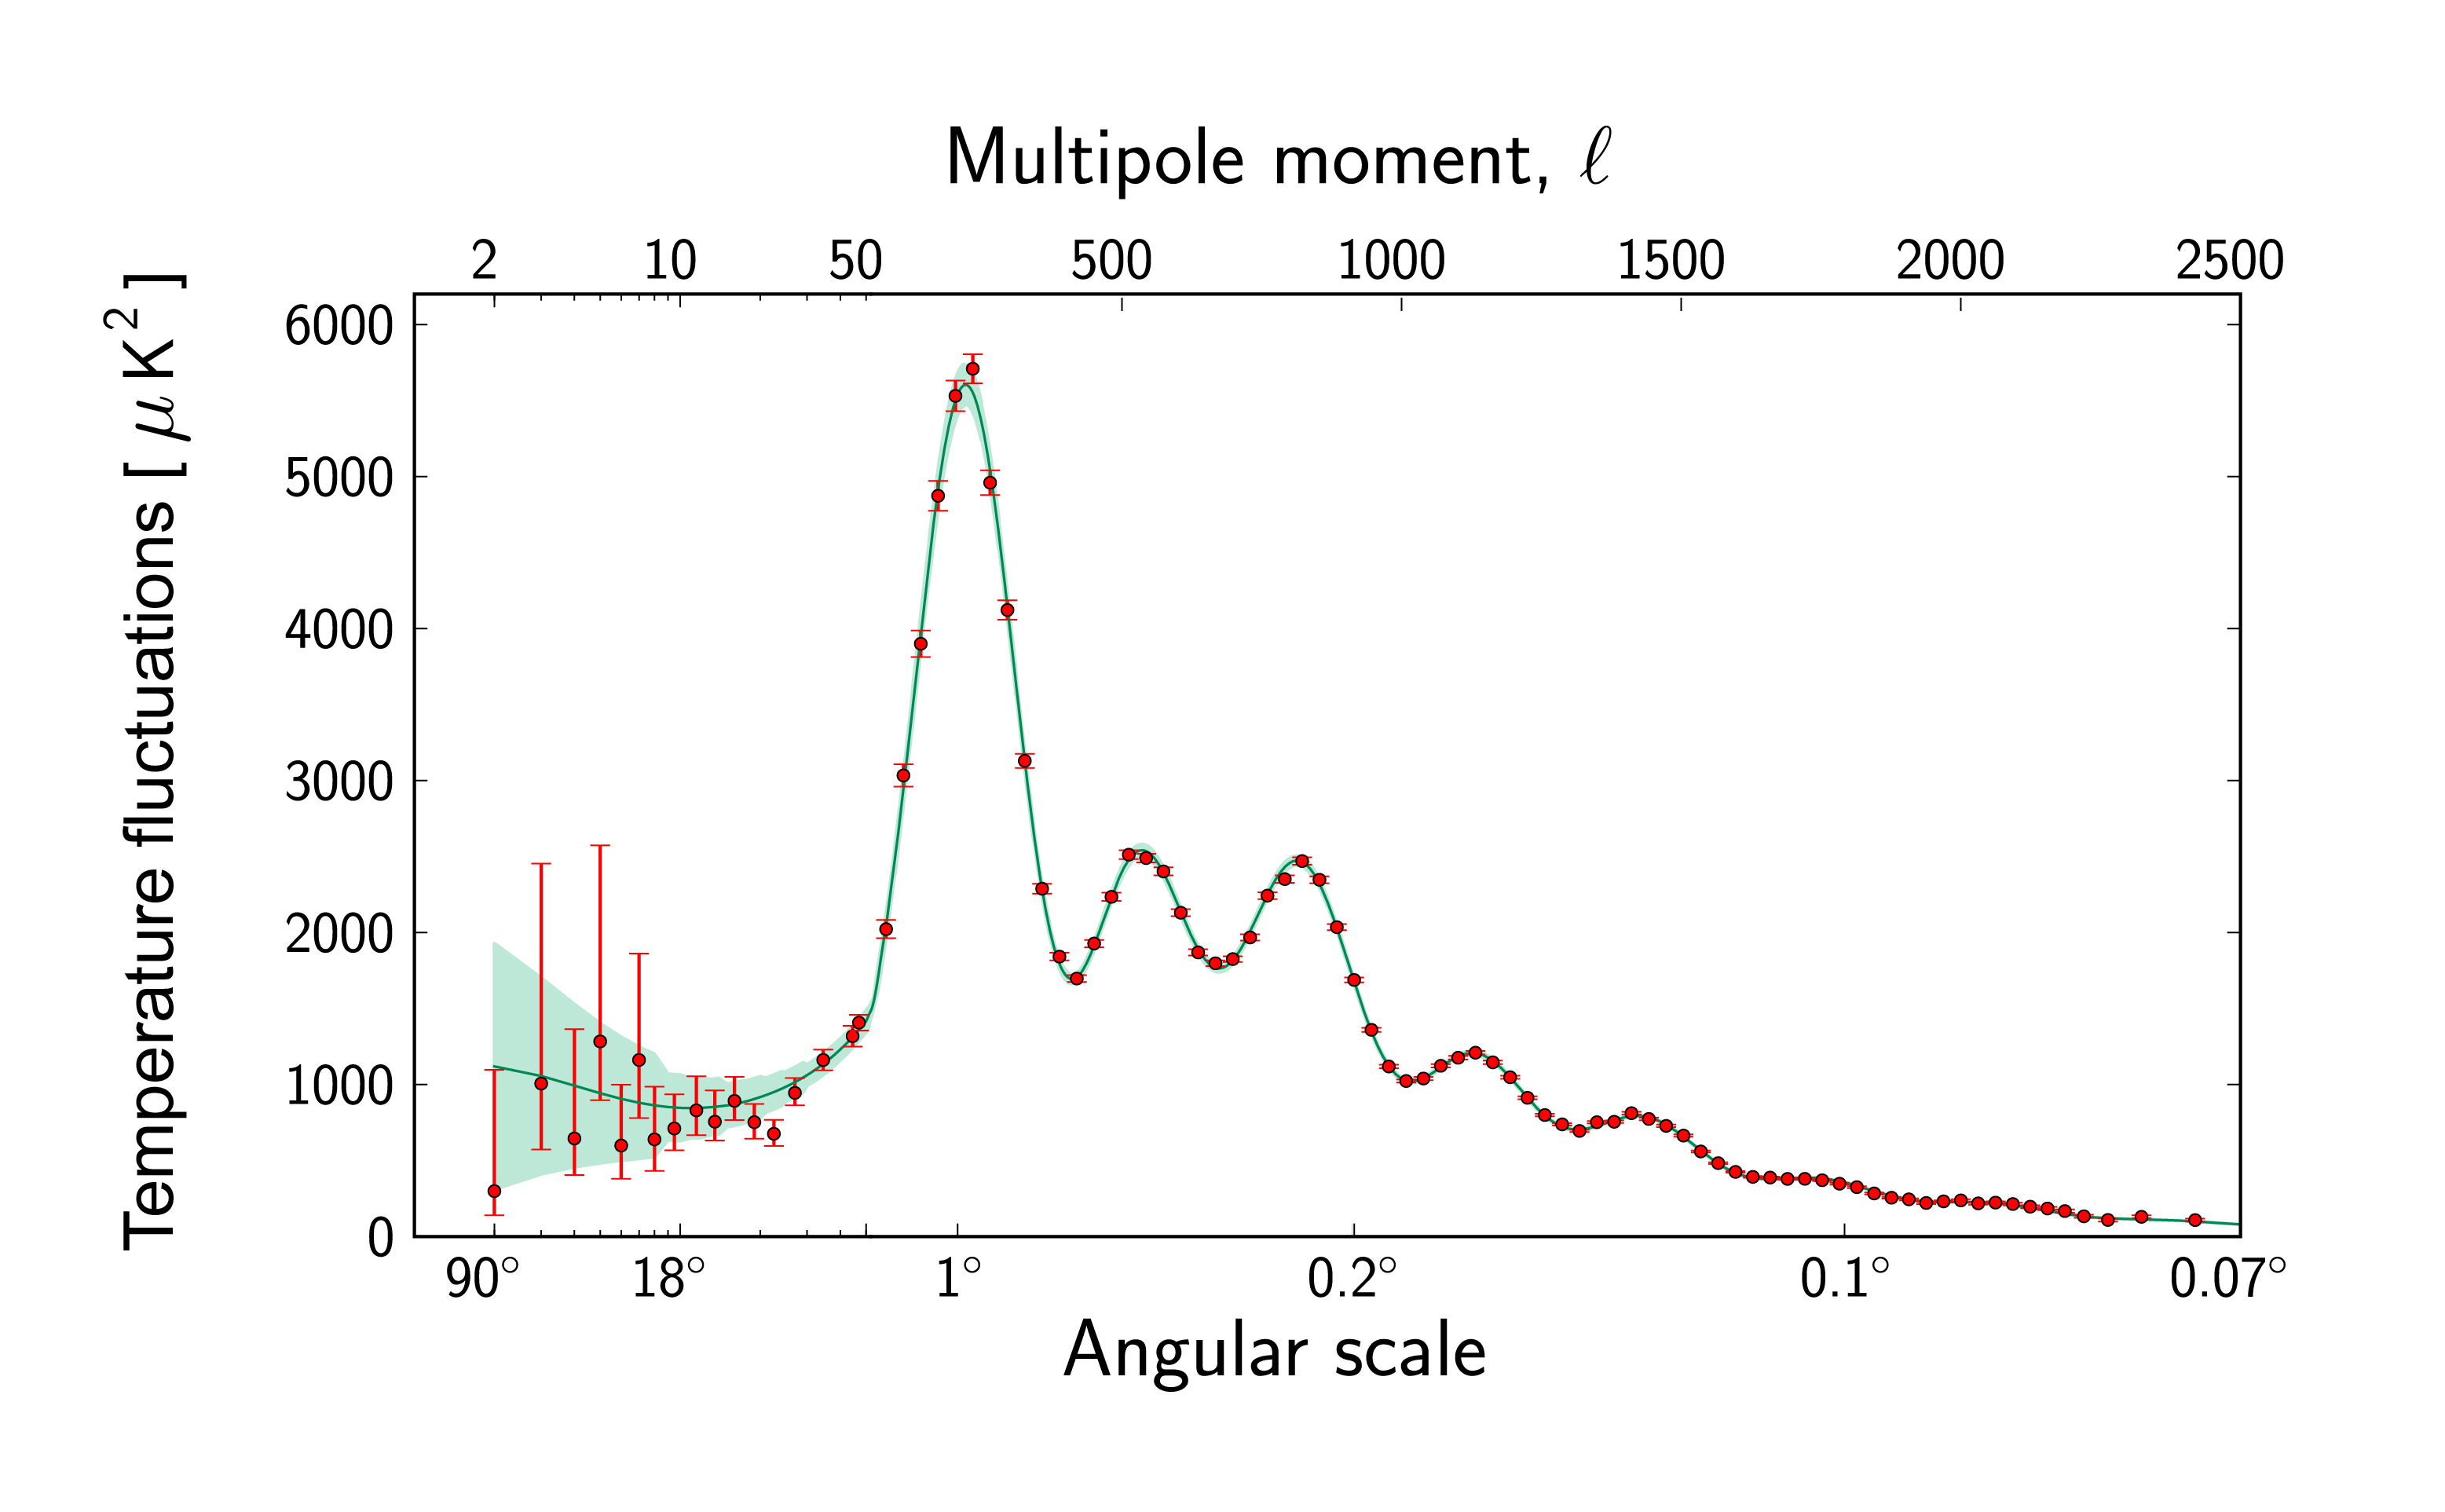
\includegraphics[width=\textwidth]{figs/planck-cmb.jpg}
        \end{column}
    \end{columns}
\end{frame}

% ── 2b. Why emulators? ─────────────────────────────────────────────────────────
\begin{frame}{Emulators in astrophysics and cosmology}
    \begin{columns}[T]
        \begin{column}{0.6\textwidth}
            \begin{itemize}
                \item Look to Neural Networks to approximate our complex astrophysical models
                \item Per parameter set run time goes from hours to
                      \textit{milliseconds}
                \item \textit{Previously infeasible inference becomes possible}
                \item Used across the field: 21-cm, CMB, SED fitting, LSS, GWs \ldots
                \item However emulators are \textit{an approximation}...
            \end{itemize}
        \end{column}
        \hfill
        \begin{column}{0.45\textwidth}
            \vspace{3em}
            \centering
            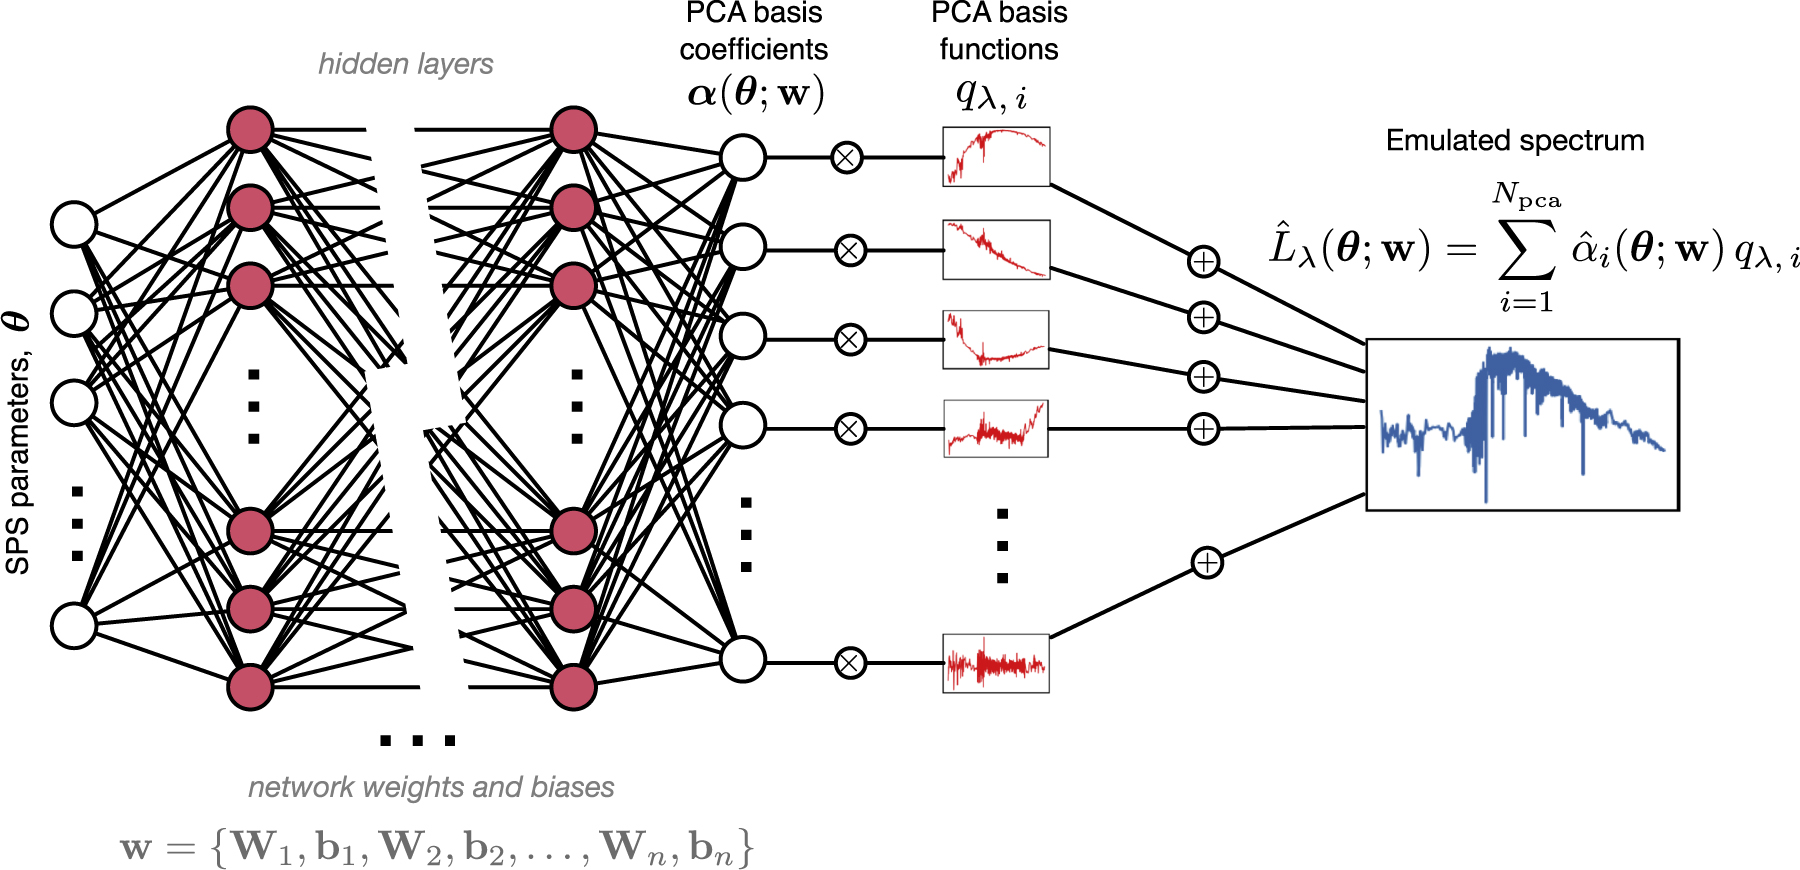
\includegraphics[width=\textwidth]{figs/speculator.jpg}
            {\footnotesize \texttt{speculator} - Alsing et al. 1911.11778}
        \end{column}
    \end{columns}
\end{frame}

% ── 3. The problem ────────────────────────────────────────────────────────────
\begin{frame}{How accurate does an emulator need to be?}
    \begin{columns}[T]
        \begin{column}{0.56\textwidth}
            \vspace{2em}
            \begin{itemize}
                \item Typically measure accuracy in \textit{signal space}:
                      \[
                          \mathrm{RMSE} = \sqrt{\frac{1}{N_d}\sum_i
                          \bigl(S_\mathrm{true} - S_\mathrm{pred}\bigr)^2}
                      \]
                \item Rules of thumb to justify, e.g.\
                      ``$\mathrm{RMSE} \lesssim 0.1\sigma$''
                \item But \textit{what does this mean for the recovered posterior?}
            \end{itemize}
        \end{column}
        \hfill
        \begin{column}{0.5\textwidth}
            %\vspace{1em}
            \centering
            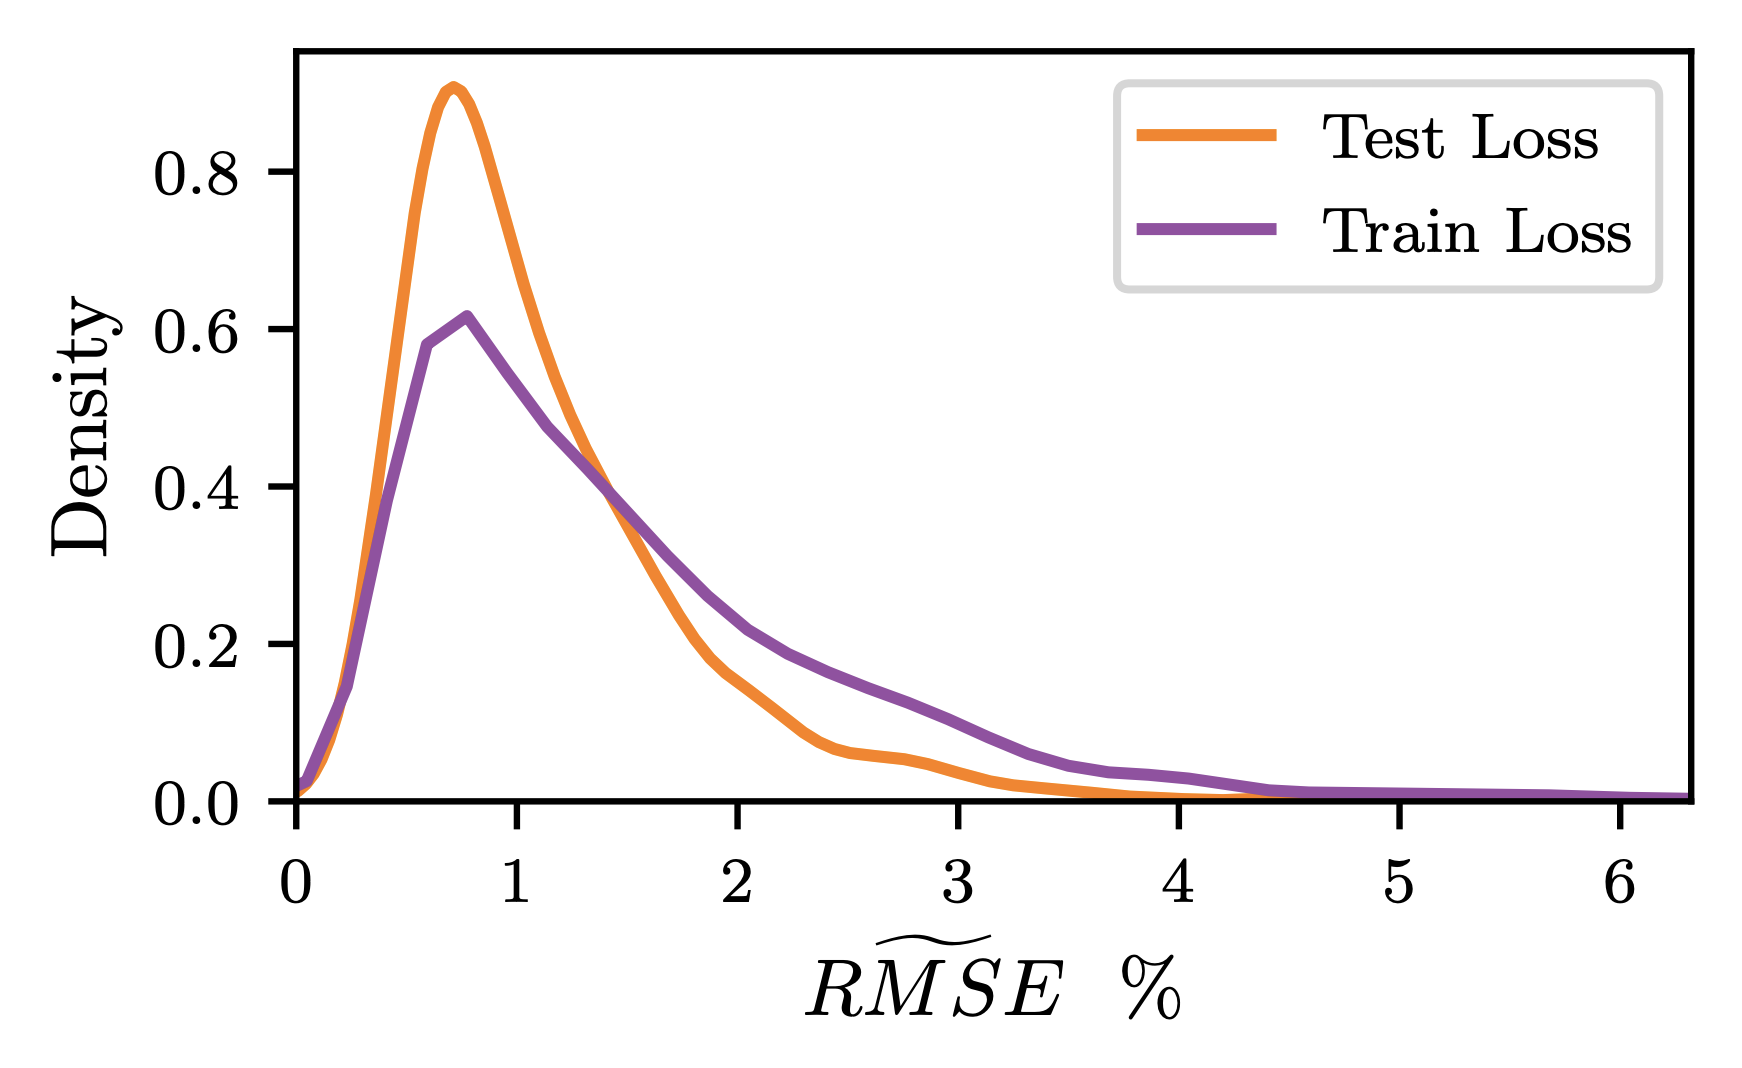
\includegraphics[width=0.7\textwidth]{figs/globalemu-error.png}\\
            {\footnotesize \texttt{globalemu} - Bevins et al. 2104.04336}\\
            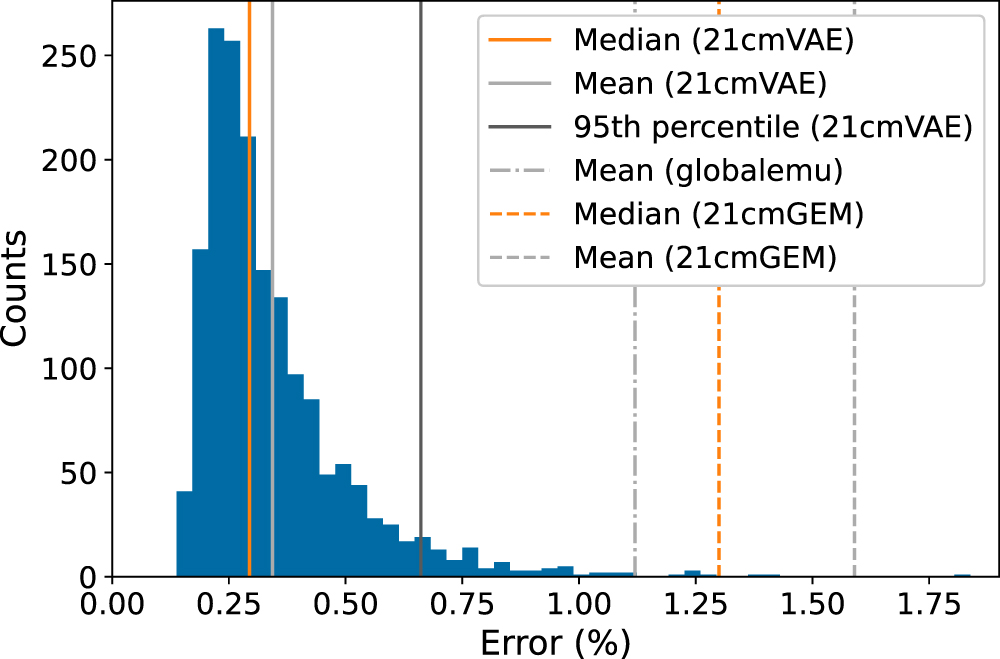
\includegraphics[width=0.7\textwidth]{figs/emulator-accuracy-21cmVAE.jpg}\\
            {\footnotesize \texttt{21cmVAE} - Bye et al. 2107.05581}
        \end{column}
    \end{columns}
\end{frame}

% ── Section divider ───────────────────────────────────────────────────────────
\sectionframe{Posterior accuracy\\\href{https://arxiv.org/abs/2503.13263}{arXiv:2503.13263}}

% ── 4a. Setting up ─────────────────────────────────────────────────────────────
\begin{frame}{Emulator error propagates into the posterior}
    \begin{itemize}
        \item Emulator error $\epsilon(\theta) = M_\epsilon(\theta) - M(\theta)$
              perturbs the log-likelihood:
              \[
                  \log L \;\longrightarrow\; \log L + \delta \log L
              \]
        \item The posterior shifts from $P(\theta|D,M)$ to $P_\epsilon(\theta|D,M_\epsilon)$:
              \[
                  P_\epsilon = \frac{L\,\pi\,e^{\delta \log L}}
                  {\int L\,\pi\,e^{\delta \log L}\,d\theta}
              \]
        \item A natural measure of the difference is the
              \textit{Kullback--Leibler divergence}:
              \[
                  \mathcal{D}_\mathrm{KL}(P \| P_\epsilon)
                  = \int P \log\!\left(\frac{P}{P_\epsilon}\right) d\theta
              \]
    \end{itemize}
\end{frame}

% ── 4b. Setting up ─────────────────────────────────────────────────────────────
\begin{frame}{Emulator error propagates into the posterior}
            \[
                  \mathcal{D}_\mathrm{KL}(P \| P_\epsilon)
                  = \int P \log\!\left(\frac{P}{P_\epsilon}\right) d\theta
              \]
    \begin{itemize}
        \item This quantifies the \textit{incorrect information inferred} (in nats)
              when using the emulator
        \item We don't have access to $P$ to evaluate this directly \ldots
        \item \ldots but we can make some progress with a few assumptions
    \end{itemize}
\end{frame}
% ── 5. Main result ────────────────────────────────────────────────────────────
\begin{frame}{A theoretically motivated upper bound}
    \begin{columns}[T]
        \begin{column}{0.5\textwidth}
            \begin{itemize}
                \item \textit{Gaussian likelihood} and broad uniform prior
                \item \textit{Linear model} around the posterior peak (similar to a Laplace approximation)
                \item \textit{White (uncorrelated) noise} in the data
            \end{itemize}
            \vspace{0.2em}
            \[
                \boxed{
                    \mathcal{D}_\mathrm{KL}(P \| P_\epsilon)
                    \leq \frac{N_d}{2}
                    \left(\frac{\mathrm{RMSE}}{\sigma}\right)^{\!2}
                }
            \]
        \end{column}
        \hfill
        \begin{column}{0.5\textwidth}
            \vspace{2em}
            \centering
            {\small For 21-cm Cosmology...}
            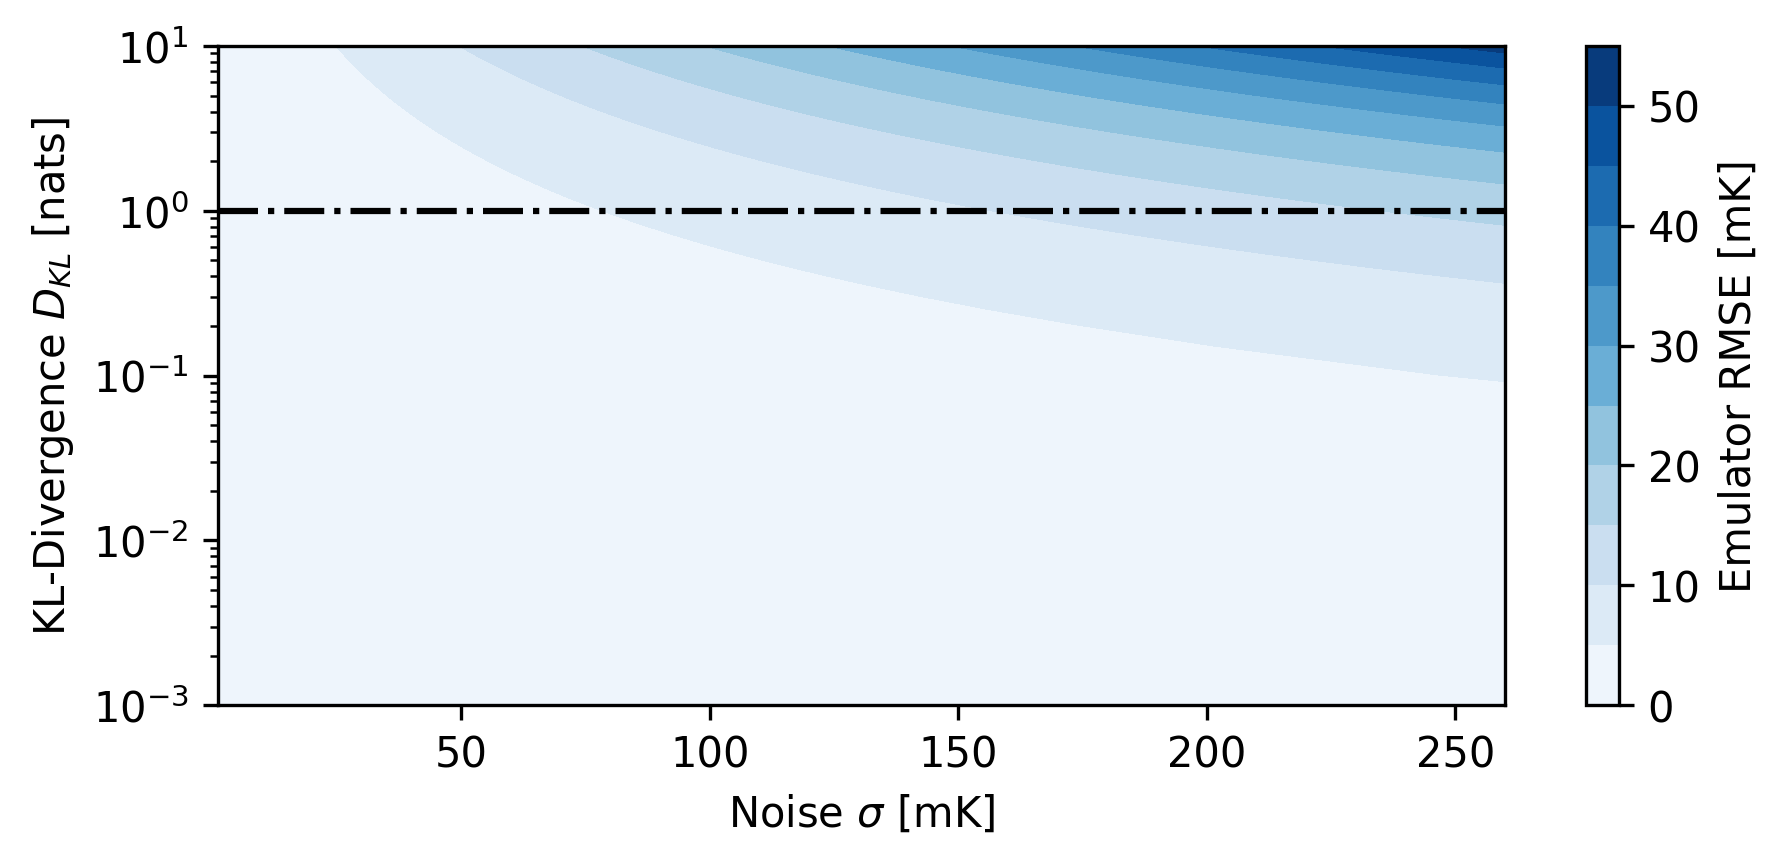
\includegraphics[width=\textwidth]{figs/kl_divergence-illustration.png}
        \end{column}
    \end{columns}
\end{frame}

% ── 6. What this gives us ─────────────────────────────────────────────────────
\begin{frame}{Why this bound is useful}
    \begin{itemize}
        \item \textit{Instrument-aware}: the required emulator accuracy scales with the
              noise -- better instruments demand more accurate emulators
        \item \textit{Predictive}: given an emulator with a given accuracy, how
              accurate can I expect my posteriors to be? 
        \item \textit{Loss function / hyperparameter tuning}: optimise emulator
              training to minimise the bound directly, instrument by instrument
        \item \textit{Broadly applicable}: SKA data analysis, SED fitting, CMB, \ldots
    \end{itemize}
\end{frame}

% ── Section divider ───────────────────────────────────────────────────────────
\sectionframe{Application to sky-averaged 21-cm cosmology}

% ── 2c. REACH ─────────────────────────────────────────────────────────
\begin{frame}{REACH -- \href{https://arxiv.org/abs/2210.07409}{2210.07409}}
    \begin{columns}[T]
        \begin{column}{0.55\textwidth}
            \begin{itemize}
                \item Dipole antenna based in the Karoo in South Africa
                \item Goal is to measure the sky-averaged 21-cm signal from neutral hydrogen
                \item Analysis pipeline heavily reliant on emulators for physical signal modelling
                \item ...and soon instrument modelling
                \item See talks from Eloy, Jacob and Sam later in the workshop
            \end{itemize}
        \end{column}
        \hfill
        \begin{column}{0.48\textwidth}
            \vspace{1em}
            \centering
            
\includegraphics[width=0.7\textwidth]{figs/reach.png}
            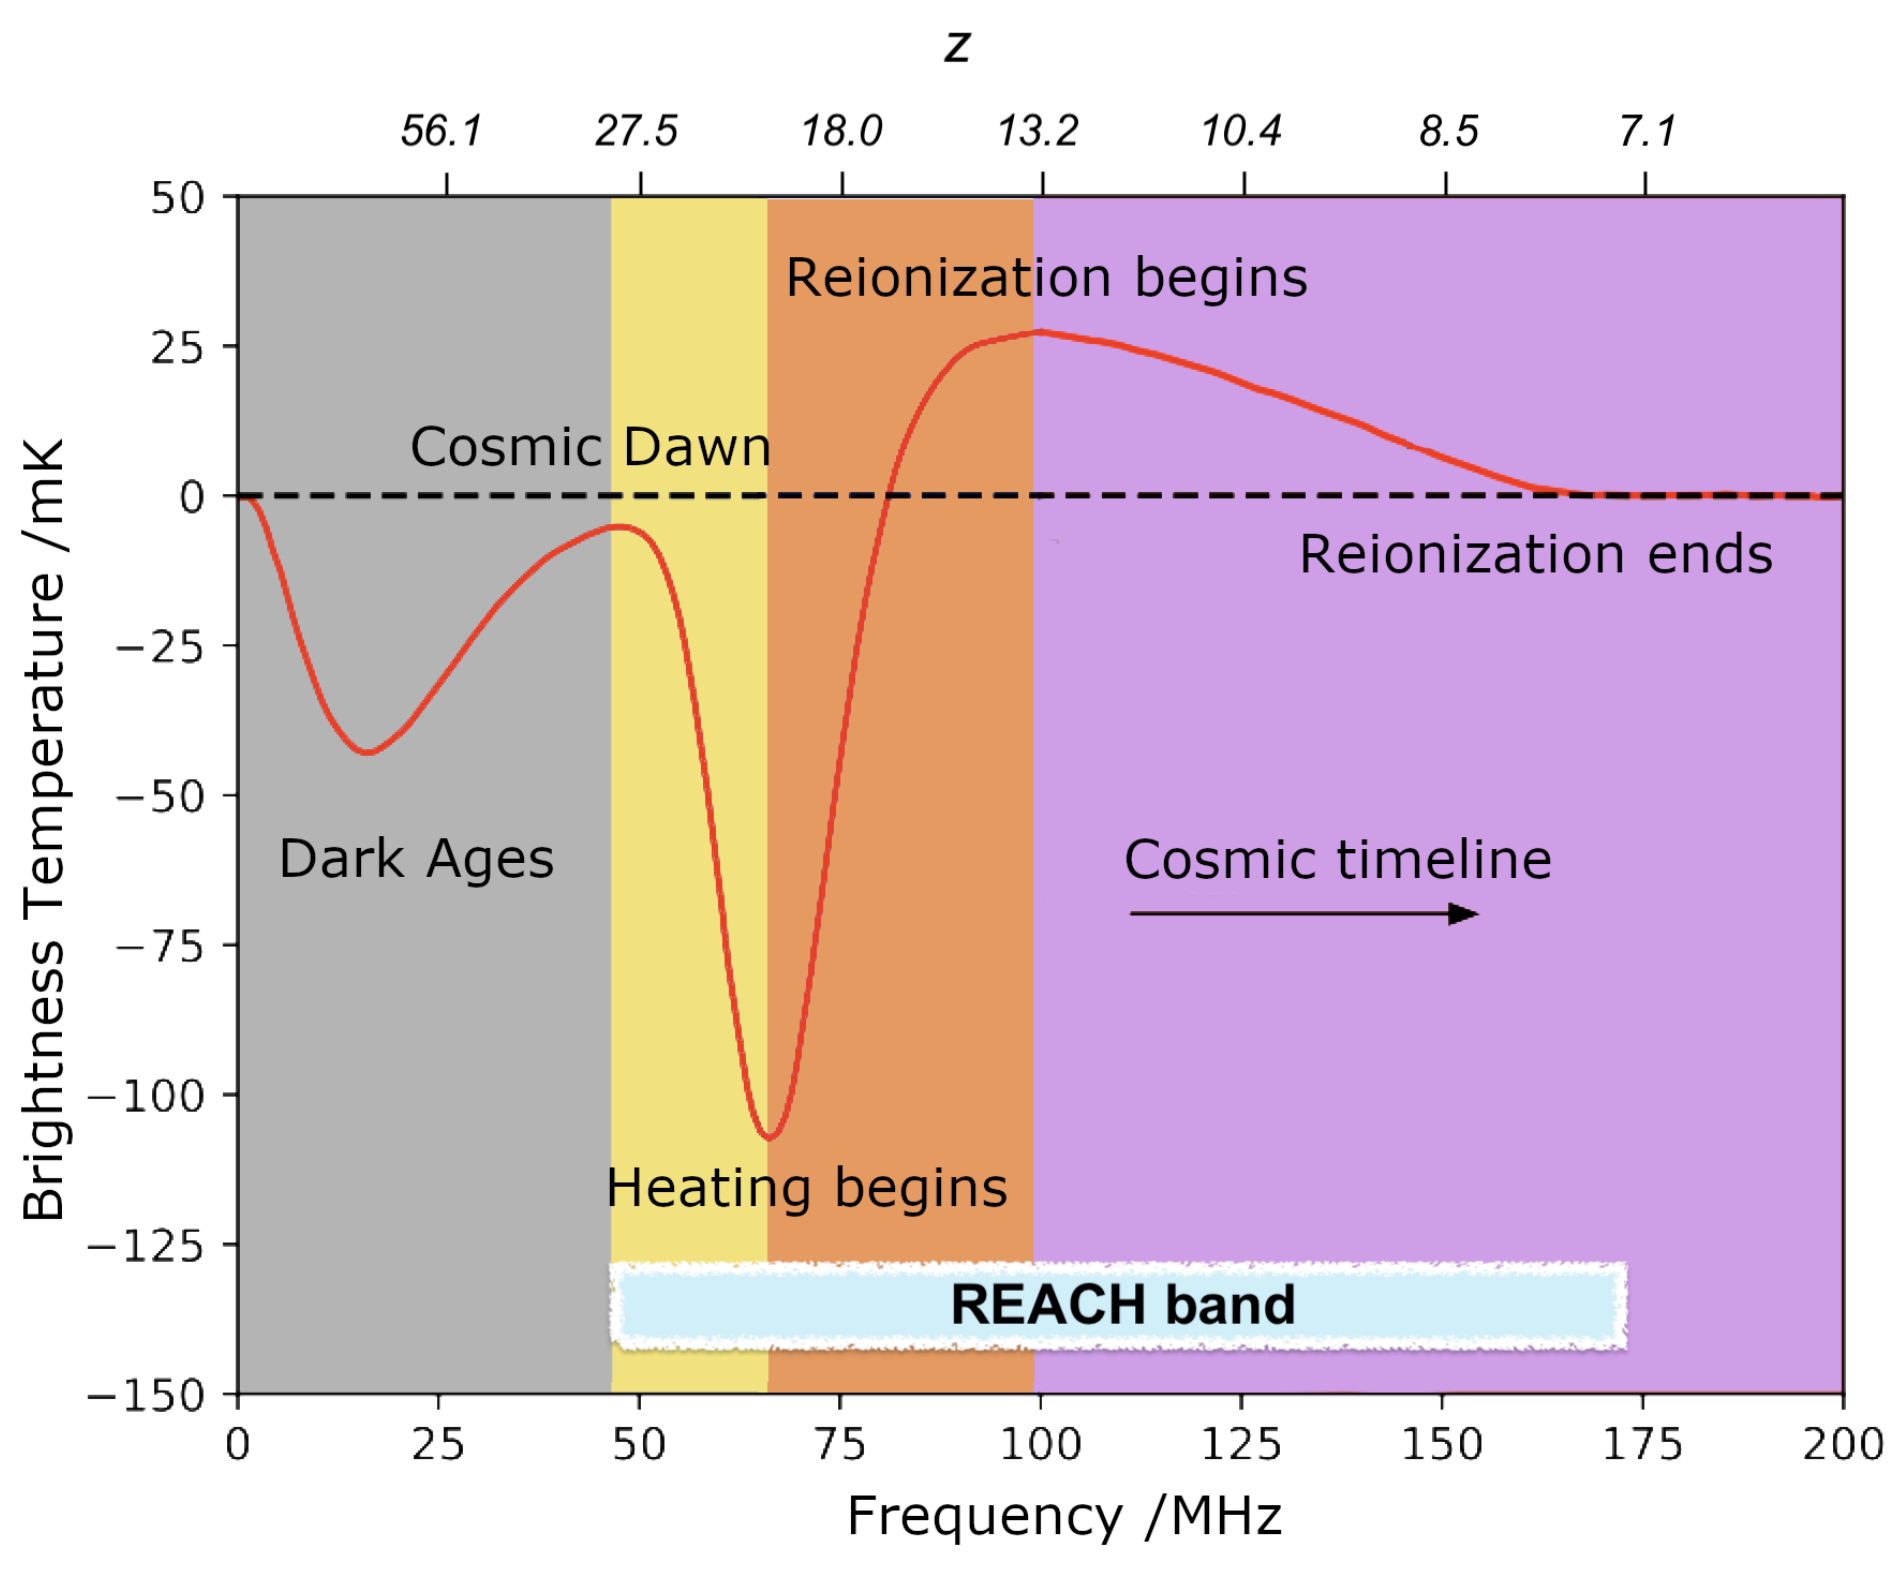
\includegraphics[width=0.75\textwidth]{figs/21cmsignal.png}
        \end{column}
    \end{columns}
\end{frame}
% ── 7. 21-cm setup ────────────────────────────────────────────────────────────
\begin{frame}{Sky-averaged 21-cm cosmology with ARES and globalemu}
    \begin{columns}[T]
        \begin{column}{0.5\textwidth}
            \begin{itemize}
                \item \textit{ARES}: 1D radiative transfer code, $\sim$seconds per
                      evaluation
                \item \textit{globalemu}: neural network emulator of ARES
                      (Bevins et al.\ 2021, MNRAS)
                \item Total of around 10,000 simulations for training, validation and testing
                \item 8 free parameters modelling reionization, X-ray heating, star formation and
                        cosmology
            \end{itemize}
        \end{column}
        \hfill
        \begin{column}{0.55\textwidth}
            \centering
            
\includegraphics[width=0.5\linewidth]{figs/globalemu.png}
            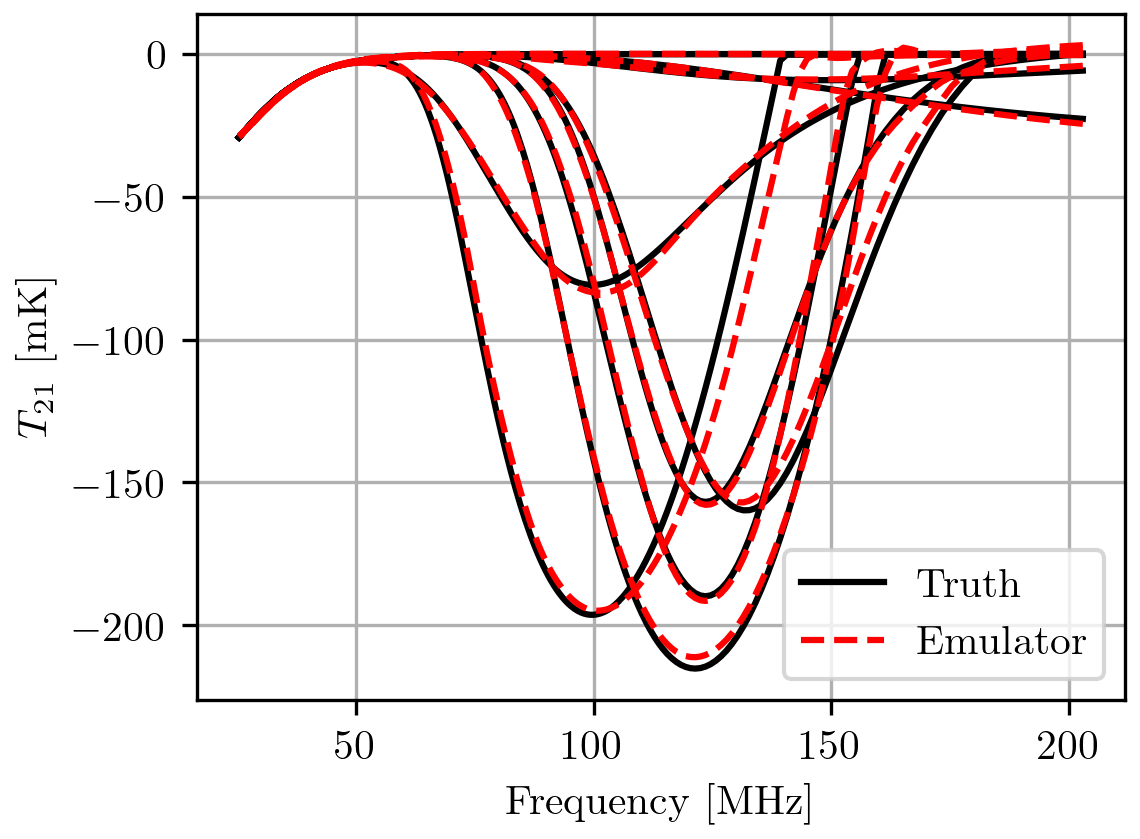
\includegraphics[width=0.65\textwidth]{figs/ares_validation_data.png}
        \end{column}
    \end{columns}
\end{frame}

% ── 8. Signal-space accuracy ──────────────────────────────────────────────────
\begin{frame}{Emulator accuracy in signal space}
        \hfill
        
        \centering
        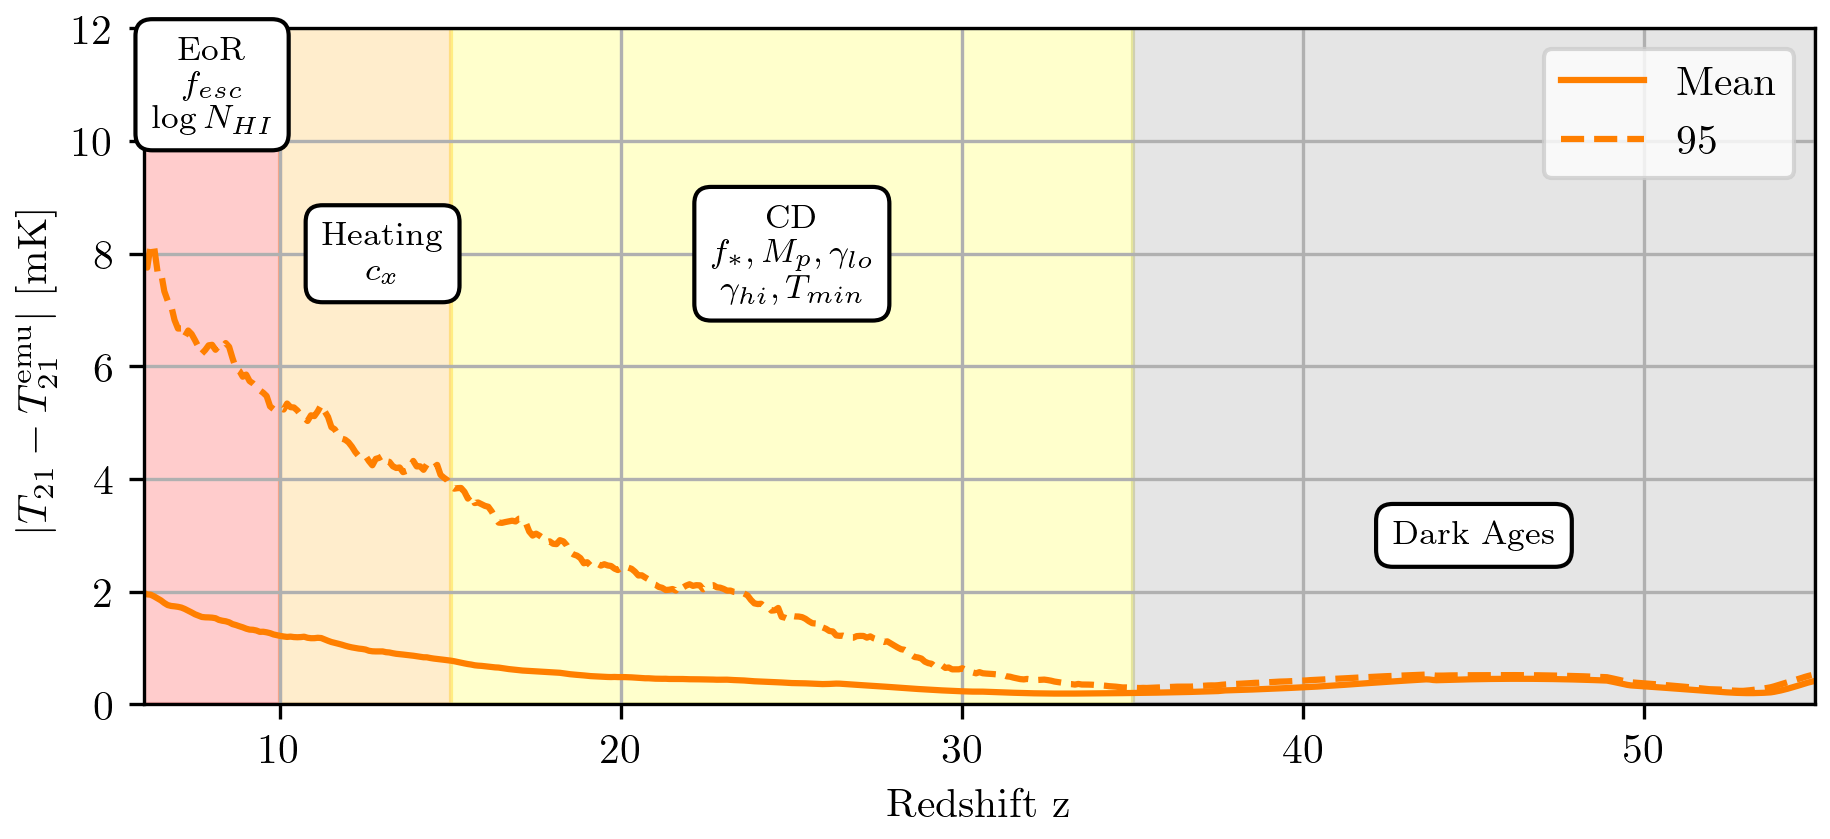
\includegraphics[width=0.8\textwidth]{figs/accuracy_comparison_ares_emulators_val_data.png}
        \\[0.3em]
        {\small Mean (solid) and 95th percentile (dashed) absolute error
        vs.\ redshift. Coloured regions: CD, Heating, EoR epochs.}
\end{frame}

% ── 10. Posterior recovery ────────────────────────────────────────────────────
\begin{frame}{Posterior recovery: ARES vs globalemu}
    \begin{columns}[T]
        \begin{column}{0.55\textwidth}
            \begin{itemize}
                \item Inference with \textsc{PolyChord} on mock data at
                      $\sigma = 5,\,25,\,50,\,250\,\mathrm{mK}$
                \item Direct comparison: posteriors from \textit{ARES} (blue)
                      vs \textit{globalemu} (orange)
                \item Posteriors agree \textit{very well} down to $\sigma = 5\,\mathrm{mK}$
                \item Estimate the KL divergence between the two distributions at different noise levels
            \end{itemize}
        \end{column}
        \hfill
        \begin{column}{0.48\textwidth}
            \centering
            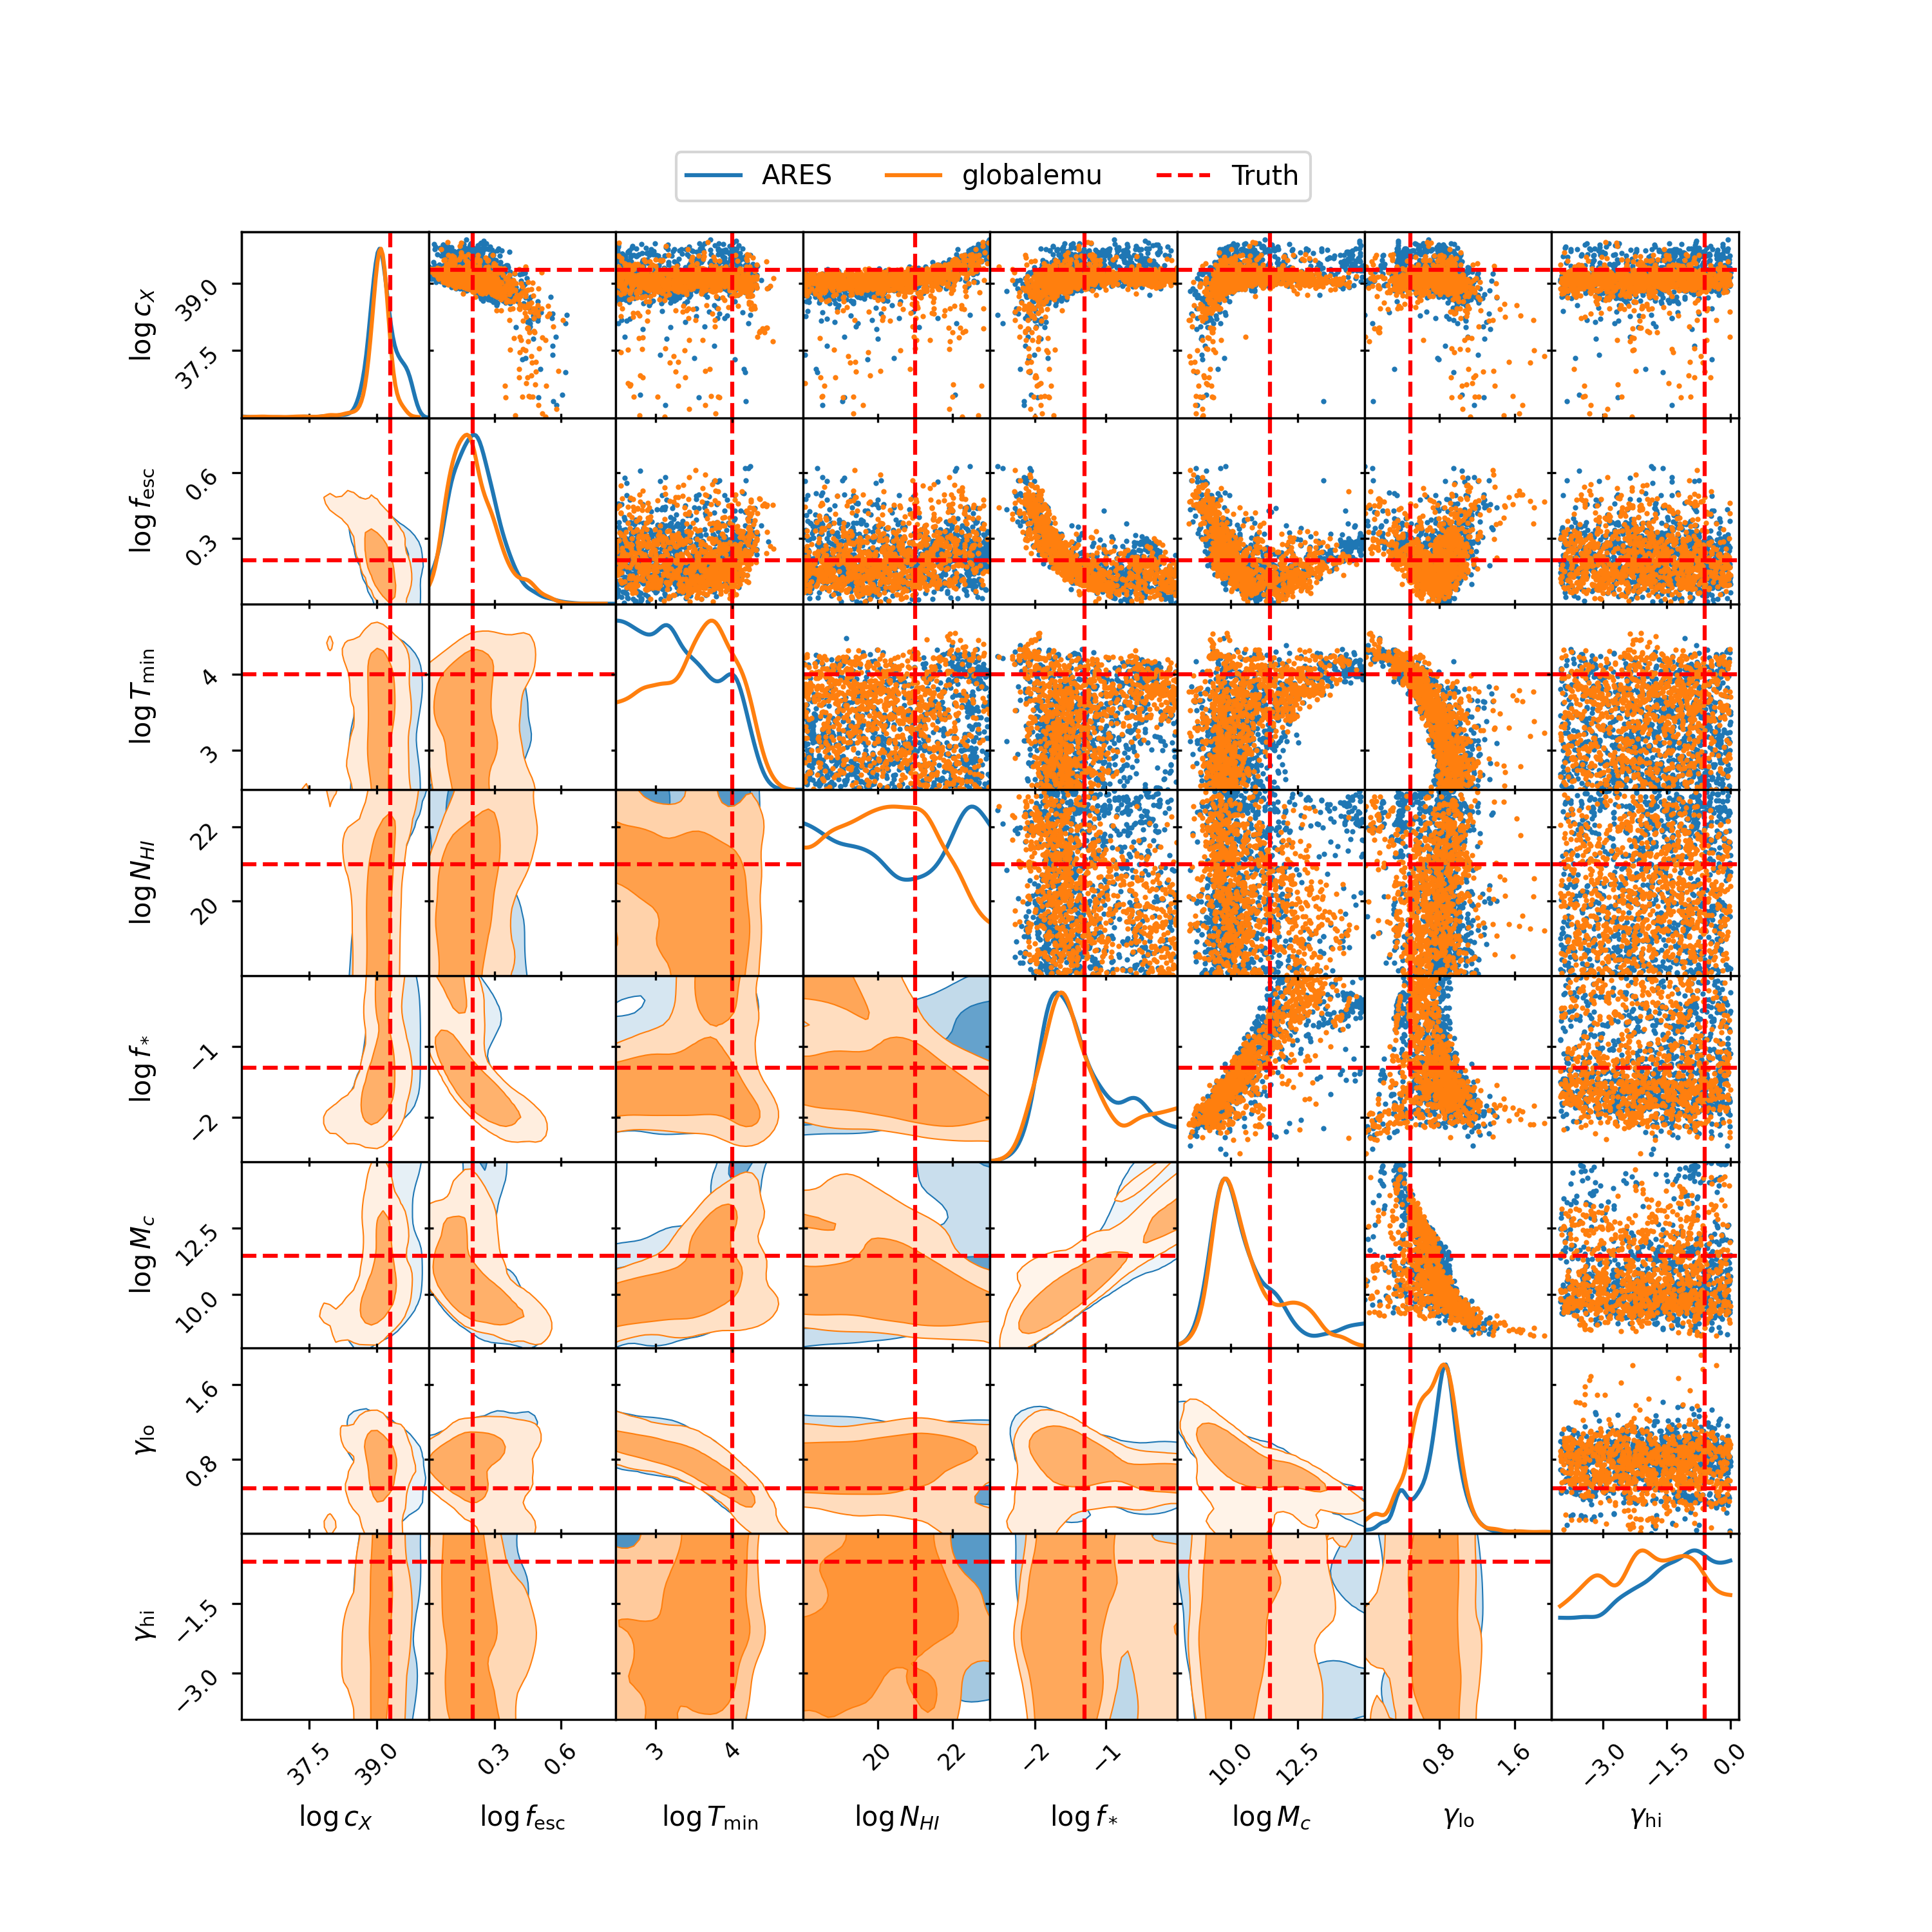
\includegraphics[width=\textwidth]{figs/posterior_ares_fiducial_model_noise_25_ARES_True_FIXED_NOISE_True.png}
            {\tiny $\sigma = 25\,\mathrm{mK}$}\\[0.1em]
        \end{column}
    \end{columns}
\end{frame}

% ── 9. KL divergence in practice ──────────────────────────────────────────────
\begin{frame}{KL divergence bound vs observed accuracy}
    \begin{center}
        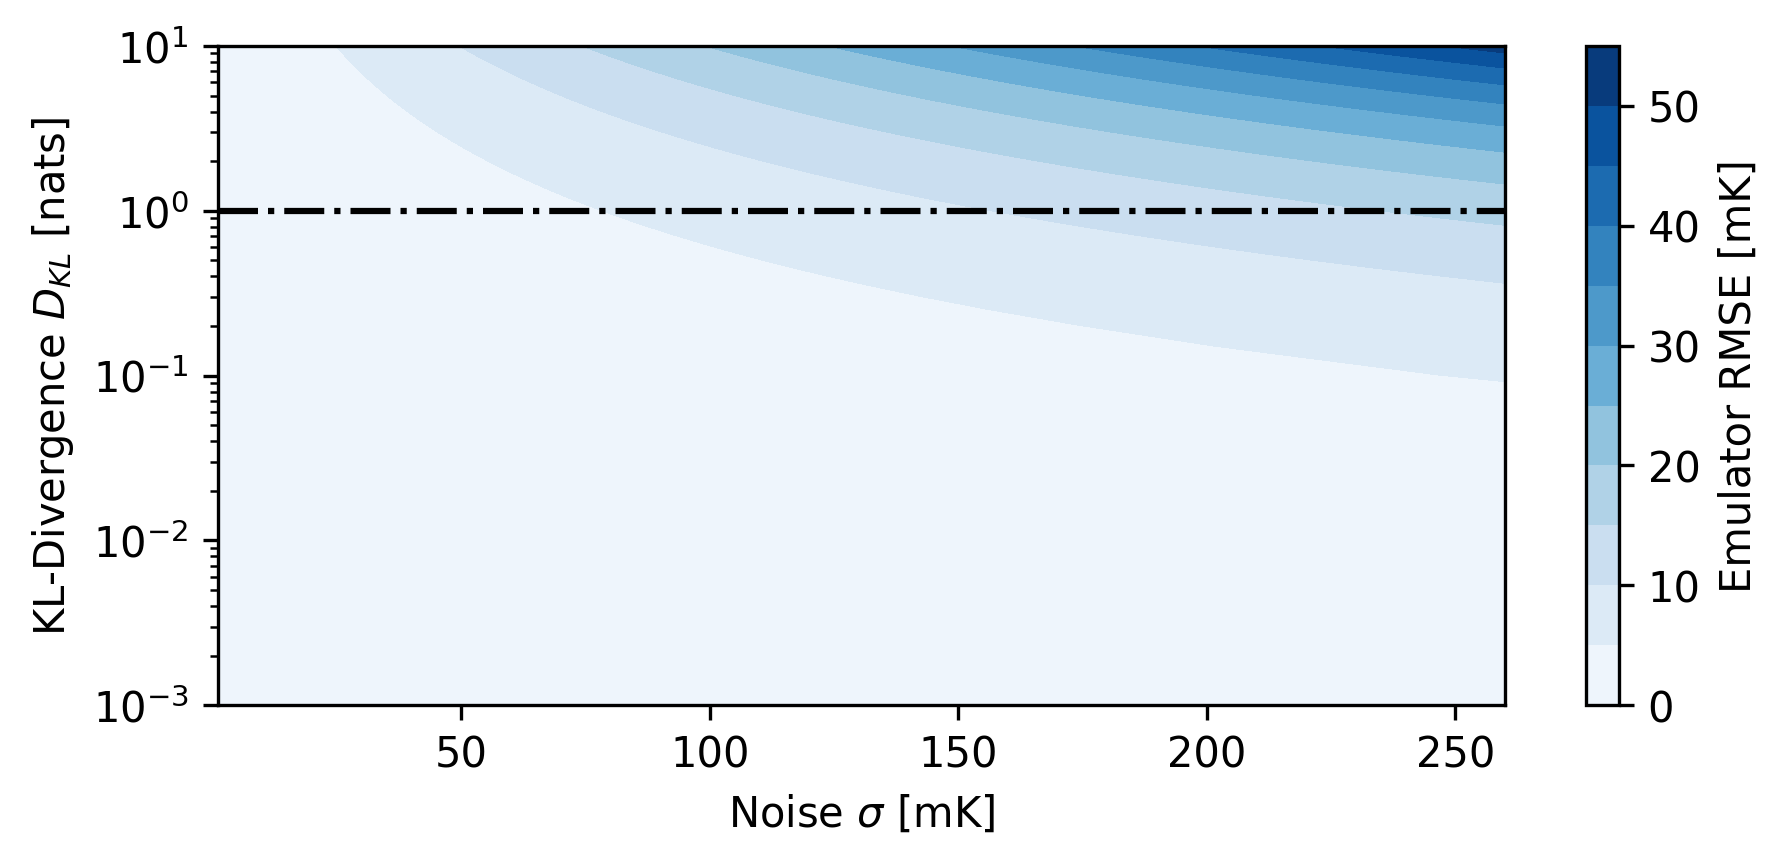
\includegraphics[width=0.7\textwidth]{figs/kl_divergence-illustration.png}
    \end{center}
    \vfill
\end{frame}

% ── 9. KL divergence in practice ──────────────────────────────────────────────
\begin{frame}{KL divergence bound vs observed accuracy}
    \begin{center}
        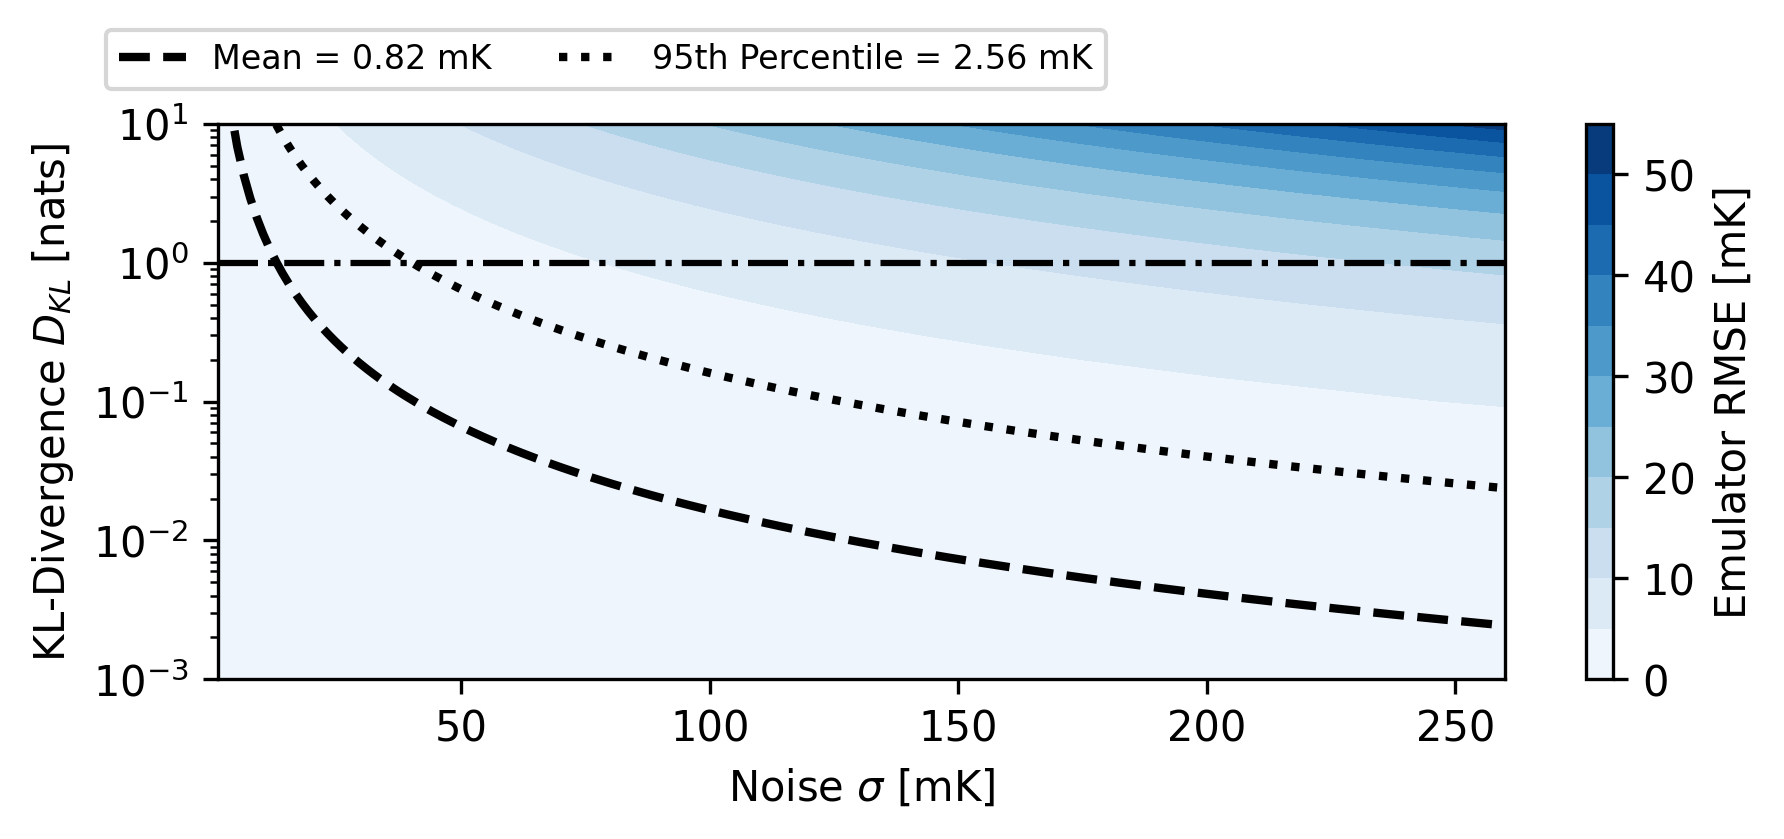
\includegraphics[width=0.7\textwidth]{figs/kl_divergence_rmse_only.png}
    \end{center}
    \vfill
\end{frame}

% ── 9. KL divergence in practice ──────────────────────────────────────────────
\begin{frame}{KL divergence bound vs observed accuracy}
    \begin{center}
        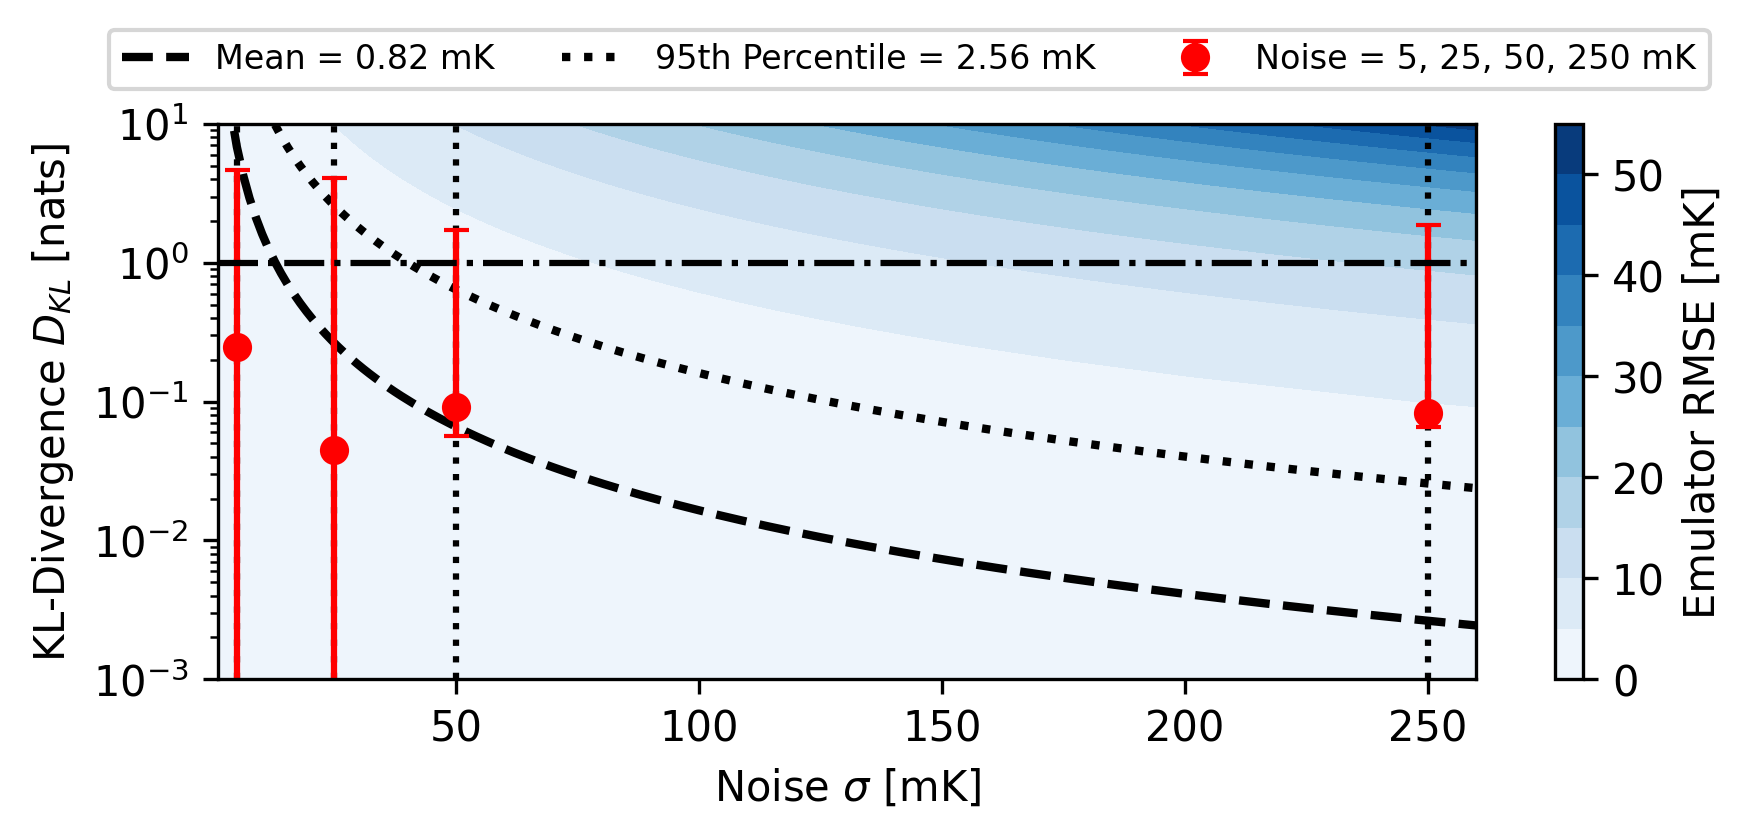
\includegraphics[width=0.7\textwidth]{figs/kl_divergence.png}
    \end{center}
    \vfill
\end{frame}


% ── 11. astroemu ────────────────────────────────────────────────────
\begin{frame}{\textsc{astroemu}}
    \begin{columns}[T]
        \begin{column}{0.52\textwidth}
            \begin{itemize}
                \item Written in JAX with JAX native dataloaders
                \item Tilling approach to emulation inspired by \textsc{globalemu}
                \item \href{https://github.com/htjb/astroemu}{github.com/htjb/astroemu}
                \item \texttt{pip install astroemu}
                \item Built in $D_{KL}(P || P_\epsilon)$ loss function
                \item Recently applied to recombination history and HYREC-2
            \end{itemize}
        \end{column}
        \hfill
        \begin{column}{0.55\textwidth}
            \centering
            
\includegraphics[width=\textwidth, height=4.cm, keepaspectratio]{figs/globalemu.png}\\[0.5em]
            \begin{minipage}{0.49\textwidth}
                \centering
                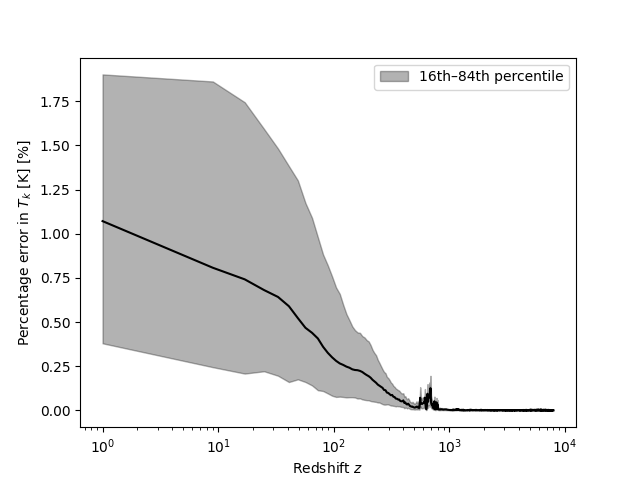
\includegraphics[width=\textwidth]{figs/hyrec_percent_error_tk.png}
            \end{minipage}
            \hfill
            \begin{minipage}{0.49\textwidth}
                \centering
                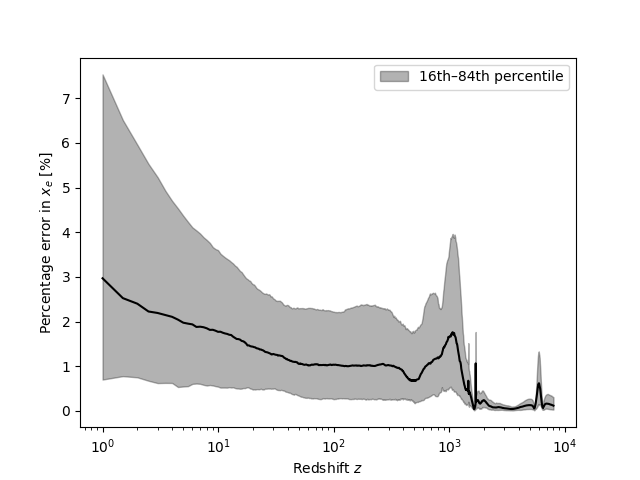
\includegraphics[width=\textwidth]{figs/hyrec_percent_error_xe.png}
            \end{minipage}
        \end{column}
    \end{columns}
\end{frame}

% ── 12. Conclusions ───────────────────────────────────────────────────────────
\begin{frame}{Summary}
    \begin{columns}[T]
        \begin{column}{0.6\textwidth}
            \begin{itemize}
                \item Upper bound:
                      $\;\mathcal{D}_\mathrm{KL} (P || P_\epsilon) \leq \frac{N_d}{2}\!\left(\frac{\mathrm{RMSE}}{\sigma}\right)^{\!2}$
                \item \textit{Instrument-aware}: better instruments need
                      more accurate emulators
                \item Need to address the assumptions we made and see if this can be generalised
                \item \textit{Broadly applicable}: any field beyond 21-cm using emulators e.g. SKA, CMB, SED fitting, \ldots
            \end{itemize}
        \end{column}
        \hfill
        \begin{column}{0.5\textwidth}
            \centering
            {\small\textit{Published in MNRAS}\\[0.2em]
            \href{https://arxiv.org/abs/2503.13263}{arXiv:2503.13263}\\[0.4em]
            \textit{Code:}\\
            \href{https://github.com/htjb/validating_posteriors}%
            {\small github.com/htjb/validating\_posteriors}\\[0.5em]
            \href{https://github.com/htjb/globalemu}%
            {\small github.com/htjb/globalemu}\\[0.5em]
            \href{https://github.com/htjb/astroemu}%
            {\small github.com/htjb/astroemu}\\[0.5em]}
            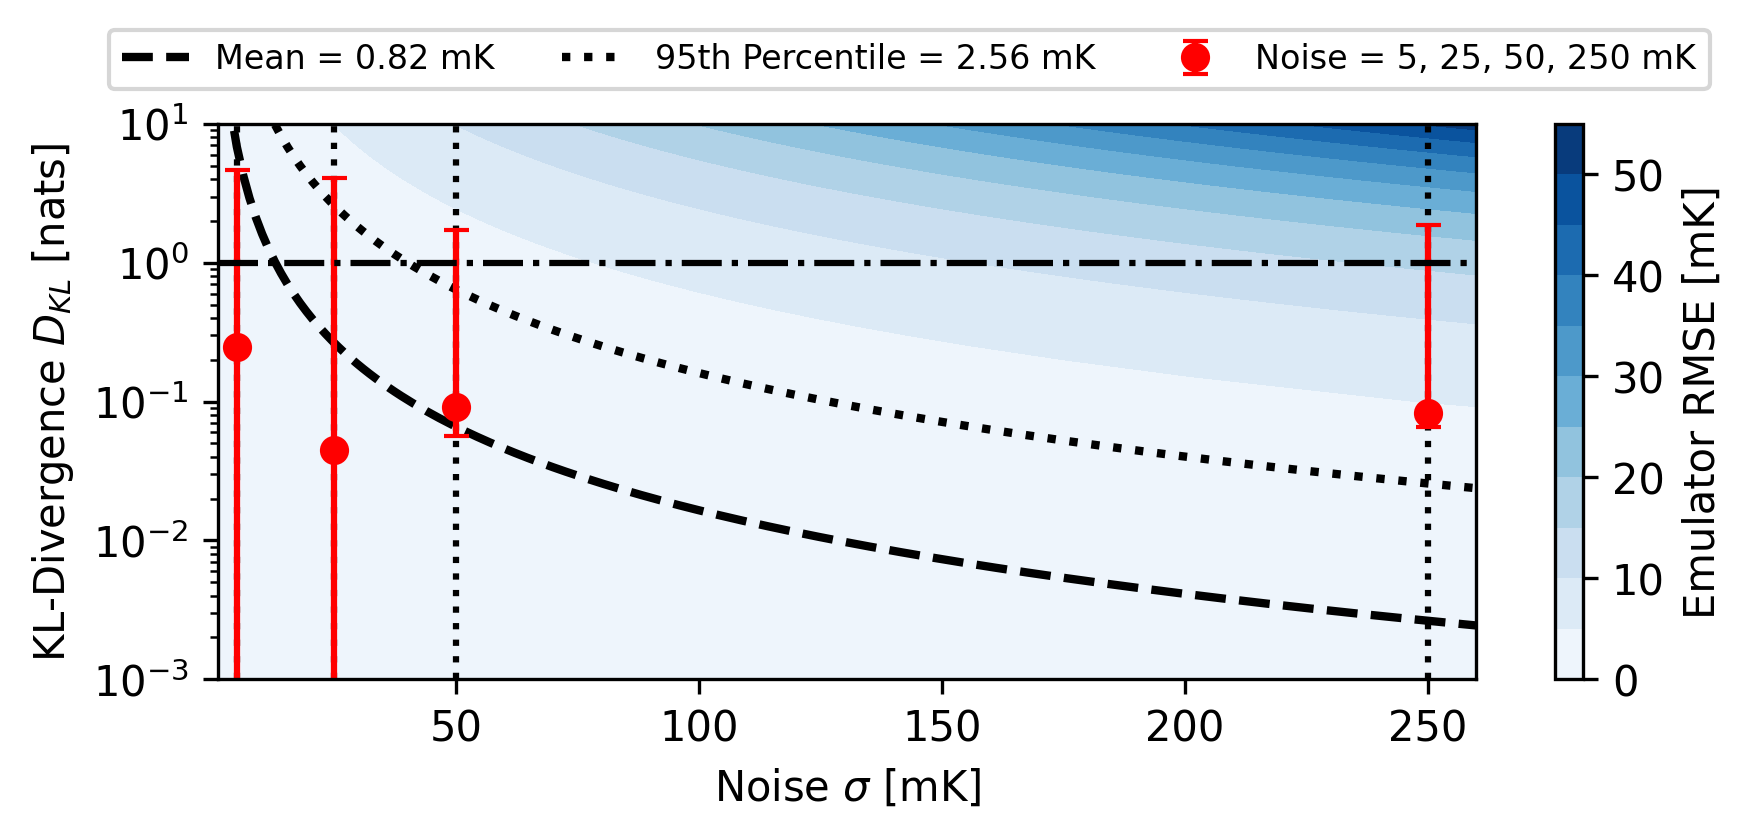
\includegraphics[width=\textwidth]{figs/kl_divergence.png}
        \end{column}
    \end{columns}
\end{frame}

% ══════════════════════════════════════════════════════════════════════════════
%  BACKUP SLIDES
% ══════════════════════════════════════════════════════════════════════════════

\sectionframe{Backup slides}

% ── B1. Derivation sketch ─────────────────────────────────────────────────────
\begin{frame}{Derivation: linear model and Gaussian likelihood}
    \begin{itemize}
        \item Assume linear model $\mathcal{M}(\theta) = M\theta + m$ and
              linear emulator error $\epsilon(\theta) = E\theta + \epsilon_0$
        \item For $E \ll M$ (slowly varying emulator error), the emulated
              posterior covariance $C_\epsilon \approx C$ and the mean shifts by:
              \[
                  \mu_\epsilon \approx \mu - C M^T \Sigma^{-1} \epsilon_0
              \]
        \item The KL divergence between two Gaussians then simplifies to:
              \[
                  \mathcal{D}_\mathrm{KL} = \tfrac{1}{2}\,
                  \epsilon_0^T \Sigma^{-1} M \!\left(M^T \Sigma^{-1} M\right)^{-1}\!
                  M^T \Sigma^{-1} \epsilon_0
              \]
        \item For white noise ($\Sigma = \sigma^2 \mathbf{1}$) this is
              $\frac{1}{2\sigma^2}\,\epsilon_0^T M M^+ \epsilon_0$
              where $M M^+$ is a projection matrix with eigenvalues in $\{0,1\}$
        \item Bounding via $\max(\lambda_n) = 1$ and $\|\epsilon_0\|^2 = N_d\,\mathrm{RMSE}^2$
              gives the limit 
    \end{itemize}
\end{frame}

% ── B2. Limitations ───────────────────────────────────────────────────────────
\begin{frame}{Limitations of the approximation}
    \begin{itemize}
        \item Assumes \textit{linearity} of the model around the posterior peak --
              may break down in high dimensions or highly curved posteriors
        \item Assumes \textit{Gaussian likelihood} -- may not hold for all
              instruments or data preprocessing choices
        \item Assumes \textit{uncorrelated (white) noise} -- extension to
              correlated noise is straightforward if $\Sigma$ is known
        \item The bound is \textit{conservative}: measured
              $\mathcal{D}_\mathrm{KL}$ values are typically well below the bound
        \item Applies most directly to posteriors that are \textit{unimodal and
              approximately Gaussian} -- multimodal cases warrant extra care
    \end{itemize}
\end{frame}

% ══════════════════════════════════════════════════════════════════════════════
\end{document}
